\documentclass[a4paper,11pt,report]{ltjsbook}
\usepackage{fancyhdr}
\usepackage[dvipdfmx]{graphicx} % for \includegraphics[width=3cm]{sample.eps}
\usepackage{times} % use Times Font instead of Computer Modern

\usepackage{hyperref}
\setcounter{tocdepth}{3}
\setcounter{page}{-1}
\usepackage{fontspec}

\usepackage[dvipsnames]{xcolor}
\usepackage{titlesec}
\definecolor{MSBlue}{rgb}{.204,.353,.541}
\definecolor{MSLightBlue}{rgb}{.31,.506,.741}
% Define a new fontfamily for the subsubsection font
% Don't use \fontspec directly to change the font
%\newfontfamily\subsubsectionfont[Color=MSLightBlue]{Times New Roman}
% Set formats for each heading level
\titleformat{\chapter}[display]
{\bfseries\HUGE\color{MSBlue}}
{\filleft\Huge\colorbox{MSBlue}{\textcolor{white}{\thechapter}}}
{-0.23em}
{\titlerule\vspace{1ex}\filright}
[\vspace{1ex}\titlerule]

\titlespacing*{\chapter}{0pt}{0pt}{30pt}
\titleformat{\section}[block]
            {\Large\bfseries\sffamily\color{MSLightBlue}}
            {\thesection}
            {1em}{}
            [\titlerule]
\titleformat*{\subsection}{\large\bfseries\sffamily\color{MSLightBlue}}
\titleformat*{\subsubsection}{\itshape\subsubsectionfont}

\renewcommand{\chaptermark}[1]{\markboth{#1}{}}

\pagestyle{fancy}
\rhead{\leftmark}
\lhead{\rightmark}

\hypersetup{
    colorlinks,
    pdfencoding=auto,
    citecolor=Sepia,
    filecolor=Sepia,
    linkcolor=Sepia,
    urlcolor=Sepia
}

%\setlength{\oddsidemargin}{0.1in}
%\setlength{\evensidemargin}{0.1in} 
%\setlength{\topmargin}{0in}
%\setlength{\textwidth}{6in} 
%%\setlength{\textheight}{10.1in}
%\setlength{\parskip}{0em}
%\setlength{\topsep}{0em}

%\newcommand{\zu}[1]{{\gt \bf 図\ref{#1}}}

\bibliographystyle{acm}

%% タイトル生成用パッケージ(重要)
\usepackage{coins-jp}

\setmainfont{IPAPMincho}
\setsansfont{MigMix 2P}
\setmonofont{Ubuntu Mono}

\usepackage{ulem}

\title{\uline{Offloading device drivers into a hypervisor for separation of concearns}}
%% 著者
\author{米司 伊織}
%% 指導教員
\advisor{筑波大二郎}

%% 専攻名 と 年月 (提出年月)
%% 年月は必要に応じて書き替えてください。
\heiseiyear{25}  % 平成の年度
%\majorfield{ソフトウェアサイエンス主専攻}
\majorfield{情報システム主専攻}
%\majorfield{知能情報メディア主専攻}

\usepackage{etoolbox}
\patchcmd{\title}{plain}{empty}{}{}

\begin{document}
\thispagestyle{empty}
\newpage
\thispagestyle{empty}
\begin{minipage}{.8\hsize}
\thispagestyle{empty}
\maketitle
\end{minipage}
\thispagestyle{empty}
\newpage

\thispagestyle{empty}
\vspace*{20pt plus 1fil}
\noindent
%%
%% 論文の概要(Abstract)
%%
\begin{center}
{\Large \bf 要  旨}
\vspace{2cm}
\end{center}

オペレーティングシステムは様々な機能を提供しているが、その中でデバイスドライバの占める開発コストは大きい。そこで本論文では、デバイスドライバを提供する低オーバヘッドのハイパーバイザと、よりシンプルなオペレーティングシステムからなる新しいオペレーティングシステムアーキテクチャ・デザインを提案し、オペレーティングシステムの開発における「関心の分離」を図る。その主要な技法としてDevice Masqueradingについて論じ、本デザインの応用について検討する。また、その評価に際して実際にBitVisorを改変して実装し、性能について実験する。また、さらにネットワーク性能を改善させる方法について議論し評価する。

keywords = {BitVisor, Hypervisor, OS Design, libraryOS, embedded computing, OS noise, open standard, virtio, paravirtual device}


%%%%%
\par
\vspace{0pt plus 1fil}
\newpage

\pagenumbering{roman} % I, II, III, IV 
\tableofcontents
\listoffigures
%\listoftables

\pagebreak \setcounter{page}{1}
\pagenumbering{arabic} % 1,2,3



\chapter{序論}

\section{背景}

\subsection{デバイスドライバの問題点}
近年、オペレーティングシステムのアーキテクチャは転換期をむかえている。その要因として、モバイル・ IoT の普及とともに、オペレーティングシステムの低消費電力化と同時に多様なデバイスに対応しなければならなくなってきているほか、ハイパフォーマンスコンピューティング環境の巨大化によって、よりオペレーティングシステムへの性能要求は高まっている。しかしながら、同時にオペレーティングシステムの開発コストは年々上がっている。その理由として、多様な SoC やデバイスの普及によって、デバイスドライバの開発コストは年々上がっているという点が挙げられる。デバイスドライバは歴史的にオペレーティングシステムの不具合の原因の最たるもので\cite{oserrors}、近年改善されているとはいえ、頻度・件数ともに主要因の一つでありつづけている\cite{faults}。また、オペレーティングシステムの開発コストもデバイスドライバは支配的な存在となっている。このことを示すためにコード行数ベースで比較すると、一例として linux の mainline(1 月 13 日時点での最新)全体に対するデバイスドライバの占める割合は 1884 万行中 1171 万行で 62.2\% となっている。この問題はデバイスドライバが各オペレーティングシステム間で再利用できないことによる。

また、ライブラリ OS の研究がここ数年で盛んになっていて実際に民用においても使われ始めているが、多くのライブラリ OS の実行環境は伝統的なオペレーティングシステムの上に限定されていて、ライブラリ OS のパフォーマンスが引き出せるとは限らない。ライブラリOSではカーネルをライブラリとしてリンクし、実行ファイルでありながら同時にオペレーティングシステムとして動作するもので、仮想化環境の中で動作させることを前提に、仮想ハードウェアの性能を引き出すことを目的にしているが、もしこれが実際のハードウェアを占有して動作することができれば、より高い性能改善が期待できる。また、コンパイルされてリンクされたライブラリOSのライブラリとアプリケーションは、様々な利点が指摘されているものの、同時に、メンテナンスするためにコンパイルしなければならないという問題点があげられる。負荷の変動によって実行環境をライブマイグレーション\cite{livemgrt}などを用いて移すことは出来るものの、通常の OS のように直接ハードウェアの上で実行するためにはそれぞれのライブラリにドライバを導入し再リンクしなければならないという困難があり、現実的ではない。%本論文で提案する Device Masquerading Underlay を用いれば、ライブラリ OS ですでに利用が進んでいる virtio という準仮想化デバイスとして実際の様々なハードウェアを利用できるようになる。

さらに、オペレーティングシステムは検証の難しい巨大なシステムソフトウェアであるので、これへの attack surface は非常に大きい。そのためオペレーティングシステムそのものが攻撃者の意図するプログラムを実行してしまう危険性が高く、オペレーティングシステムがデバイスへ直接アクセスできる場合にはデバイスを破壊したり、デバイスを乗っ取って攻撃者にとって都合がよい動作をさせる可能性がある。例えば、キーボード入力を取得し送信するプログラムを隠蔽して動作したり\cite{thinkpadkeyvlnt}、バッテリーのファームウェアに侵入し発火・爆発させることや\cite{macbookbatvlnt}、起動できなくさせること\cite{takekoshinvmvlnt}が可能となる。

\section{提案}

上記の問題はデバイスドライバの共有化が進んでおらず、それぞれのオペレーティングシステムでデバイスドライバの開発を別々に行わなければならないという点や、それぞれのデバイスがそれぞれのアクセスメソッドを持っていて、統一化されていないという点によって生じている。そこでデバイスドライバをハイパーバイザにオフロードすることで、オペレーティングシステムの開発という、様々な機能の実装を連携して進めなければならなかったものからデバイスドライバの開発を分離し関心の分離を図る。また、この分離によって、仮にオペレーティングシステムの脆弱性を利用して任意の特権コードが実行できるようになっても実デバイスの代わりに仮想デバイスを提供していることによって実際の有効な破壊を未然に防ぐことができるようになる。

そのために本論文では Device Masquerading という技法とそれを利用したハイパーバイザを提案し、これを利用し、包括的に捉えた新しいオペレーティングシステムアーキテクチャについて議論する。

具体的には、オペレーティングシステムの機能を、デバイスドライバのようなハードウェアとのインターフェース部分と、ファイルシステムやプロセス管理などのソフトウェア部分を分離し、前者を Device Masquerading Underlay, 後者を Function Kernel と呼ぶ。この二つは virtio と呼ばれる共有メモリのリングバッファの標準規格を通して通信する。
Device Masquerading Underlay は Function Kernel に対して非依存であるため、これが提供するデバイスドライバを複数のオペレーティングシステムが利用できるようになる。
また、 virtio という標準規格を用いるので既存のオペレーティングシステムがそのまま Function Kernel として利用できる。
さらに、この実装を Parapass-through Hypervisor である BitVisor を元に行い、性能評価を行う。

\chapter{設計と技法}

\section{Device Masquerading Underlay の提供するドライバの定義}

デバイスドライバの再利用については、 Le Vasseur らの論文\cite{reuse}で提案された手法が興味深い。これもデバイスドライバの再利用を仮想化技術を用いて行うことで、ターゲットにするオペレーティングシステムにデバイスドライバを搭載せず、オペレーティングシステム非依存の形でデバイスドライバを利用できるというものだ。この論文では、ターゲット環境はホスト環境にあり、デバイスドライバを提供する層がその上でゲスト環境として動作するというアーキテクチャが提案されている。この論文でも仮想化とメモリ機構を利用し十分に高速に動作するほか、この論文での利点として、ゲスト環境でドライバを提供するオペレーティングシステムは既存のものを拡張したものなので、既に市場で使われているデバイスドライバが利用できるという点があげられる。しかし、デバイスドライバとしてオペレーティングシステムをゲスト環境で動作させることによるフットプリントが大きくなることが予想されるほか、ドライバを提供されるオペレーティングシステムが仮想化をサポートしないとならない。

ユーザのオペレーティングシステムに制限や新たな必要要件を与えずにデバイスドライバを提供するには、ユーザのオペレーティングシステムよりも先に起動したほうがよい。そこで、デバイスドライバを提供するソフトウェアをハイパーバイザとして実装し、ユーザのオペレーティングシステムをその後起動することにした。このソフトウェアを Device Masquerading Underlay と呼び、後者のユーザのオペレーティングシステムを便宜的にFunction Kernelと呼ぶことにする。

Device Masquerading Underlay は Function Kernel に対して非依存なデバイスドライバを提供するが、同時に自身がデバイスドライバを提供しないデバイスについては Function Kernel からの操作を許したい。これによって、 Device Masquerading Underlay が提供できるデバイスがあまり多くない状況から本研究で提案するアーキテクチャを採用することが出来、スムーズな移行が可能になる。

そこで Device Masquerading Underlay と Function Kernel のアクセスするそれぞれのデバイスについて考えることにする。

実際にマシンに存在するハードウェアの集合を $ Dev_{real} $ 、 Device Masquerading を施す機能を関数 $ M(x) $と表記するとする \ref{mudef} 。

また、 $M$ の定義域を $ Dev_{hyp\_can\_drive} $ とかくとする\ref{mdef}。

\begin{eqnarray}
M(x) & := & x を Device Masquerade する\label{mudef}\\
M & : & Dev_{hyp\_can\_drive} \vdash Dev_{kernel}\label{mdef}
\end{eqnarray}

すると、 Function Kernel が発見できるデバイスのリストは以下のようになる \ref{kerndef}。

\begin{equation}
Dev_{kernel} = map(M, Dev_{real} \times Dev_{hyp_can_drive}) \oplus (Dev_{real} \backslash Dev_{hyp\_can\_drive}) \label{kerndef}
\end{equation}

このように、 Device Masquerading Underlay に対応するドライバがないデバイスは Function Kernel に直接渡される。このことを実現するために、$Dev_{kernel}$ と $Dev_{real}$ はどちらもデバイスの集合でなければならない。ということは、関数 $M$ はデバイスを受け取ってデバイスを返す関数となる。通常のデバイスドライバはデバイスを操作してソフトウェアのインターフェースを提供するが、 Device Masquerading Underlay はデバイスを操作しつつ、デバイスのように振る舞う必要がある。

通常のオペレーティングシステムに内蔵されたデバイスドライバは、オペレーティングシステムの他の機能と関数呼び出しを用いて通信するので、オペレーティングシステムの実装や ABI に依存してしまうというだけでなく、この手法では Device Masquerading Underlay の機能を実装できないことになる。そこで本研究では、 Device Masquerading Underlay をハイパーバイザとして実装し、 Function Kernel は仮想化されたゲスト環境の上で動くとし、 Device Masquerading Underlay は一般の仮想化技術を用いて仮想化されたデバイスを提供することとする。この時、この Underlay がドライバを持っていないデバイスはそのままゲスト環境に提供するようにするため、 Parapass-through \cite{bitvisor} という技術を用いる。

Device Masquerading Underlay はハイパーバイザとして実装されるので、 Function Kernel が起動する前に Device Masquerading Underlay が起動する必要がある。そして、自身がデバイスドライバを持っているデバイスのみ初期化し、後述する Device Masquerading を施す。そして残りのデバイスとともにこれらをゲストに提供するために、 parapass-through 技術を用いる。

\section{Device Masquerading}
%\subsection{Device Masqueradingのコンセプト}

Parapass-through Hypervisor は一般のハイパーバイザとは異なり、ほとんどのデバイスをゲスト OS に提供する。一般のハイパーバイザは、管理者 OS の上で動作し、ゲスト OS には自身のデバイスを提供しない。例えば Xen では Dom0 が実際のデバイスを動作させ、 DomU の環境でデバイスが必要になった場合には、DomU の OS に含まれた専用デバイスドライバが XenBus などを通して仮想デバイスあるいは準仮想化デバイスを動作させ、 Dom0 がこれによって必要になる I/O をエミュレートし再現する\ref{existhyp}。また、 QEMU+KVM においても、仮想デバイスか準仮想化デバイスをホストのプロセスとして動作する QEMU がエミュレートし、カーネルがゲスト OS をアプリケーションとして処理し、管理する。一方、 Parapass-Through Hypervisor の実装である BitVisor ではホスト OS を含むアービテータが存在せず、ただ一つのゲスト OS のみが常に動作する。ハイパーバイザは介入が必要な例外が発生した場合に限り最小限動作し、必要がない限り、実在するデバイスへのアクセスをゲスト OS に許している。これにより不必要なエミュレーションコストを排除でき、ハイパーバイザによる余分なコストが非常に小さくなっている\cite{bitvisor}。

Device Masquerading とは、実デバイスへのアクセスをハイパーバイザがゲスト OS に提供許可する代わりに、ハイパーバイザ自身が実デバイスのアクセスを行い、リクエストされた情報を高速なリングバッファであるvirtio\cite{virtio}を通してゲスト OS と通信するというものだ。

ここで、既存のハイパーバイザによる準仮想化と本研究で提案する Device Masquerading との違いを説明する。

上述のように、既存のハイパーバイザではアクセスに要するパスが多い上に管理用のオペレーティングシステムが必要になる\ref{existhyp}。それに対し、 bitvisor のような parapass-through hypervisor ではデバイスを pass-through することができるうえ、デバイスへのアクセスの途中で介入しデータを改変することが出来るが、実デバイスのドライバがゲスト OS に必要だった。

\begin{figure}[htbp]
  \begin{minipage}{0.5\hsize}
    \begin{center}
      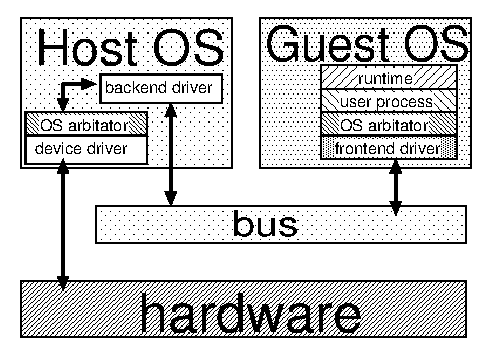
\includegraphics[width=\textwidth]{./xen.eps}
      \caption{既存のハイパーバイザ(ここでは Xen) でのデバイスアクセス}
      \label{existhyp}
    \end{center}
  \end{minipage}
  \begin{minipage}{0.5\hsize}
    \begin{center}
      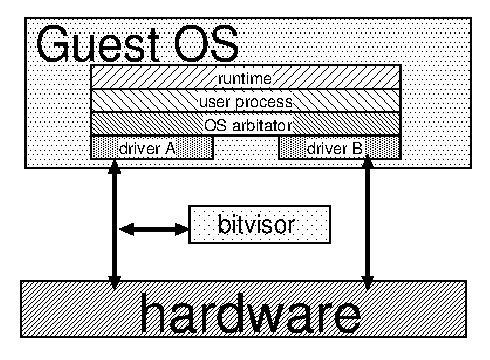
\includegraphics[width=\textwidth]{./bitvisor.eps}
      \caption{parapass-through hypervisor でのデバイスアクセス}
      \label{bitv}
    \end{center}
  \end{minipage}
\end{figure}

それに対し、 Device Masquerading を行う小さなハイパーバイザ ( ここでは Device Masquerading Underlay と呼ぶ ) を導入すると、ゲスト OS ( ここでは Function Kernel と呼ぶ ) には実デバイスの制御を行う必要性がなく\ref{underlayarch}、オペレーティングシステムに求められる他の機能の開発に注力できる。 Function Kernel はそれぞれのデバイスクラスに対してただ一つのデバイスドライバさえあればよく、この一つのドライバをすべてのユーザが使ううえ、このドライバは実デバイスを扱わないため、ドライバのカバレッジが高く堅牢になる。%XXX

Device Masquerading Underlay はオペレーティングシステム非依存なため、より多くのユーザが使用でき、より検査されるほか、より多くの開発リソースが期待でき、またそのメリットは複数のオペレーティングシステム開発者に還元されることになる。

\begin{figure}[htbp]
  \begin{minipage}{0.5\hsize}
  \begin{center}
    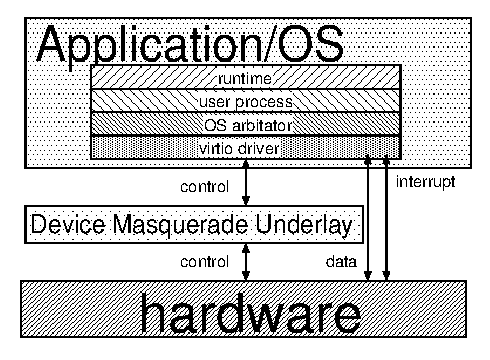
\includegraphics[width=\textwidth]{./underlay.eps}
    \caption{提案手法と伝統的なオペレーティングシステムを組み合わせたデバイスアクセス}
    \label{underlayarch}
  \end{center}
  \end{minipage}
  \begin{minipage}{0.5\hsize}
  \begin{center}
    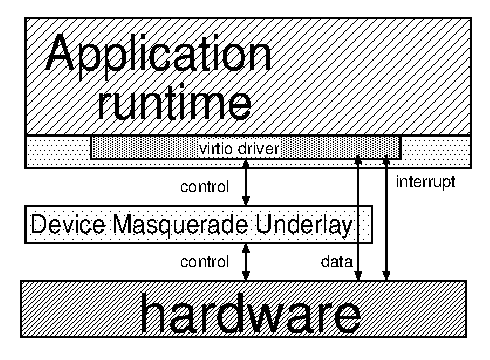
\includegraphics[width=\textwidth]{./underlay_unikernel.eps}
    \caption{提案手法と Unikernel を組み合わせたデバイスアクセス}
    \label{unduni}
  \end{center}
  \end{minipage}
\end{figure}

具体的な実装として、おもに Device Masquerading Underlay は 2つの部分からなる。
第一に、実際のデバイスを制御したり、デバイスとやりとりする部分である。第二に、virtio デバイスとして振る舞う部分である。

virtio デバイスとして振る舞う部分は共通のコードを使うことができ、デバイス固有のドライバ部分のみをそれぞれ作成すればよい。この二つのコミュニケーションは Device Masquerading Underlay の内部のバッファを用いて行う。

\begin{figure}[htbp]
  \begin{center}
    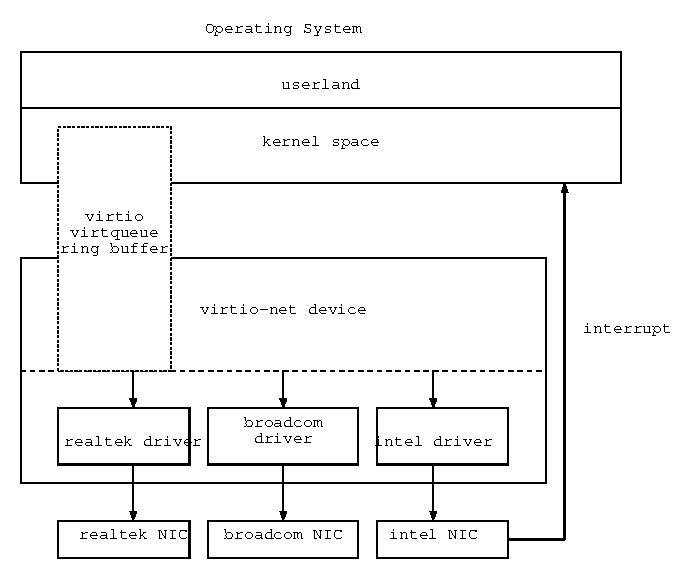
\includegraphics[width=.7\textwidth]{./archtech.eps}
    \caption{Device Underlay Architechture}
    \label{underlayarch}
  \end{center}
\end{figure}


\section{Zero-copy Device Masquerading}

Device Masquerading Underlay は実際のデバイスを制御しつつ、 virtio というデバイスがそこに実在しているかのように見せることで実現とするが、これだけでは性能的な困難が解消できない。そこで本章では、オーバヘッドの解消のための技法を提案する。

まず大きな性能改善の妨げとして、メモリコピーの速度の問題があげられる。オペレーティングシステムは多くの場合、通信の内容を書き込んだメモリの in-kernel buffer をリングバッファとしてデバイスに提供することで高速に通信しているが、図 \ref{underlayarch} のようなアーキテクチャでは、 virtio デバイスとして振る舞う箇所と個別のデバイスドライバの箇所でも同様にバッファを用いてやり取りする。これは不要なコピーが余計に増えていることになる。もっとも遅い箇所は後述のようにデバイスへのコミュニケーションだが、 virtio 化の部分に限るともっとも遅い箇所はメモリコピーであった。

そこでメモリコピーを減らし、不可欠なデバイスへのコピーを除いてメモリコピーを最終的にはゼロにしたい。この手法を独自に Zero-copy Device Masquerading と名付け実装する。図で示すと図 \ref{underlayzerocpy}のようになる。

この技法の概要は、主に Function Kernel から与えられたメモリバッファをそのままデバイスへ書くというものだが、そのためには個別のデバイスドライバが virtio 特有の処理を行わなければならず、図 \ref{underlayarch} で表したような分離が難しくなる。そこで個別のデバイスドライバでの virtio 対応を極力減らすために実装上の工夫が必要となった。

\begin{figure}[htbp]
  \begin{center}
    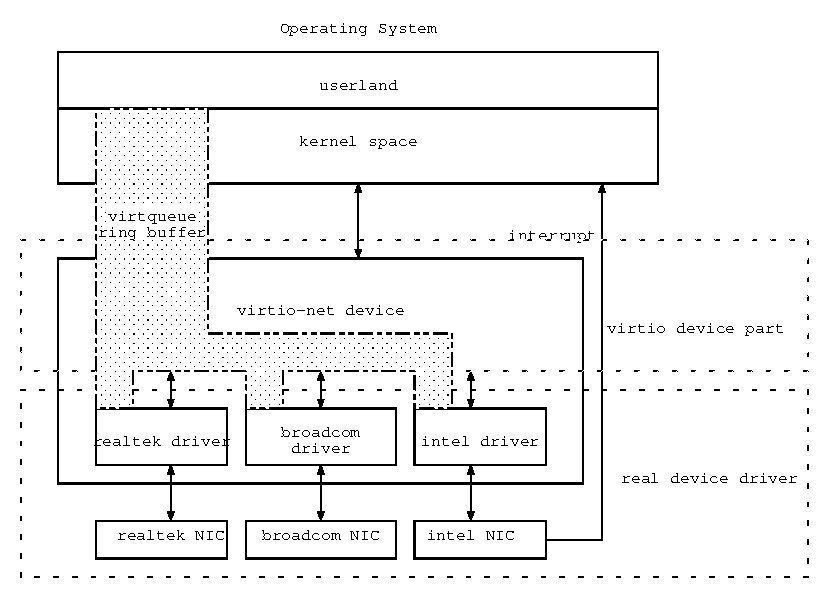
\includegraphics[width=.7\textwidth]{./underlayzerocpy.eps}
    \caption{Device Underlay Architechture}
    \label{underlayzerocpy}
  \end{center}
\end{figure}


%\section{Exitless Device Masquerading}

\chapter{実装}

\section{Device Masquerading Underlay の技術的仕様}

Device Masquerading Underlay の仕様は上記のとおりだが、実装上の制約をいくつか述べる。まず前述のように必須な処理としてOSより先に起動するという点が挙げられる。ここで行う処理は主に、 Device Masquerading Underlay のプログラム領域の保護や、 virtio 化のためのフック関数の登録、virtio 化するためのデバイスの検索と初期化である。

\subsection{Device Masquerading Underlay の隠蔽}

まず自らの隠蔽について述べる。

Function Kernel はどの領域に Device Masquerading Underlay があるのか調べる方法がないので、メモリ領域全体に書き込みを行いかねない。また、自らが管理しているはずのメモリ領域に書いた場合、正しく読み出せなければならない。であるから、 Device Masquerading Underlay はそもそも Function Kernel が書き込まず、また万一書いたとしても書いたとおりに正しく読み出せなくてもよい特別な領域を作って「潜む」必要がある。そのような領域として ACPI テーブルの末尾が挙げられる。

ACPI テーブルとは、電源管理やデバイスツリーの管理のために用意されたメモリ領域で、プラットフォームに非依存の標準規格で定められたものである。 ACPI テーブルはファームウェアによって提供されるが、この領域も Device Masquerading Underlay と同じく上書きされてはならないメモリ領域で、だが Device Masquerading Underlay とは異なり、自らの領域を OS に通達することができる。そこで BitVisor では ACPI テーブルの領域を取得後、その領域に続く場所に自らのプログラムをコピーしなおす。このように起動中の処理として自らのプログラムを再配置する処理は既存のオペレーティングシステムでも一般的な技法である。しかし BitVisor がこれらとは異なるのは ACPI テーブルの直後の箇所に再配置するという場所の差異の他に、ACPI 領域を取得するオペレーティングシステムの操作をインターセプトして、自らの領域を含めた「より大きい」領域がまるで ACPI テーブル領域として予約されているかのように振る舞うという点となる。このように確保したメモリ領域にオペレーティングシステムが読み書きしようとした場合は無効になり、常に 0 が読み出されるようになっている。このことを可能にするのは SPT または EPT という技術である。この技術については後述する。

Device Masquerading Underlay も BitVisor の技法を踏襲し、 EPT およびメモリマップの構造を取得する命令のインターセプトを用いて Function Kernel からの破壊を防ぎ、セキュリティを担保している。

\subsection{適切なデバイスドライバの検索とハンドリング関数への関連付け}

\section{EPTによるフックの動作}
\section{virtio の仕様について}
\section{PCI device discoveryについて}
\section{virtqueue の仕様について}
\section{virtio-net の仕様について}

\section{Exitless Device Masquerading の仕組み}
\section{送信時の動作}
\section{受信時の動作}
\section{制御}


\chapter{評価}

\chapter{結論}

\chapter{Appendix}

\bibliography{main}

\end{document}
